%%%%%%%%%%%%%%%%%%%%%%%%%%%%%%%%%%%%%%%%%%%%%%%%%%%%%%%%%%%%%%%%%%%%%%%%%%%%%%%%
%2345678901234567890123456789012345678901234567890123456789012345678901234567890
%        1         2         3         4         5         6         7         8

\documentclass[letterpaper, 11 pt, conference]{ieeeconf}  % Comment this line out
                                                          % if you need a4paper
%\documentclass[a4paper, 10pt, conference]{ieeeconf}      % Use this line for a4
                                                          % paper

\IEEEoverridecommandlockouts                              % This command is only
                                                          % needed if you want to
                                                          % use the \thanks command
\overrideIEEEmargins
% See the \addtolength command later in the file to balance the column lengths
% on the last page of the document



% The following packages can be found on http:\\www.ctan.org
\usepackage{graphicx}
%\usepackage{epsfig} % for postscript graphics files
%\usepackage{mathptmx} % assumes new font selection scheme installed
%\usepackage{times} % assumes new font selection scheme installed
%\usepackage{amsmath} % assumes amsmath package installed
%\usepackage{amssymb}  % assumes amsmath package installed
\usepackage{cite}
\usepackage{tikz}

\title{\LARGE \bf
Predicting Yelp Star Reviews Based on Network Structure with Deep Learning}

%\author{ \parbox{3 in}{\centering Huibert Kwakernaak*
%         \thanks{*Use the $\backslash$thanks command to put information here}\\
%         Faculty of Electrical Engineering, Mathematics and Computer Science\\
%         University of Twente\\
%         7500 AE Enschede, The Netherlands\\
%         {\tt\small h.kwakernaak@autsubmit.com}}
%         \hspace*{ 0.5 in}
%         \parbox{3 in}{ \centering Pradeep Misra**
%         \thanks{**The footnote marks may be inserted manually}\\
%        Department of Electrical Engineering \\
%         Wright State University\\
%         Dayton, OH 45435, USA\\
%         {\tt\small pmisra@cs.wright.edu}}
%}

\author{Luis A. Perez$^{1}$% <-this % stops a space
\thanks{$^{1}$L. Perez is an MS Candidate in the School of Engineering at Stanford University,
        450 Serra Mall, Stanford, CA 94305, USA
        {\tt\small luis0 at stanford.edu}}%
}


\begin{document}



\maketitle
\thispagestyle{empty}
\pagestyle{empty}


%%%%%%%%%%%%%%%%%%%%%%%%%%%%%%%%%%%%%%%%%%%%%%%%%%%%%%%%%%%%%%%%%%%%%%%%%%%%%%%%
\begin{abstract}

In this paper, we tackle the real-world problem of predicting Yelp star-review rating based on business features (such as images, descriptions), user features (average previous ratings), and, of particular interest, network properties (which businesses has a user rated before).

In recent years, breakthroughs in deep learning have led to increased accuracy in commong supervised learning tasks, such as image classification, captioning, and language understanding. However, the idea of combining deep learning with network feature and structure appears to be novel. While the problem of predicting future interactions in a network has been studied at length, these approaches have often ignored either node-specific data or global structure \cite{PintrestProject}.

We demonstrate that taking a mixed approach combining both node-level features and network information can effectively be used to predict Yelp-review star ratings. We evaluate on the Yelp dataset by splitting our data along the time dimension (as would naturally occur in the real-world) and comparing our model against multiple baseline models from literature.

\end{abstract}


%%%%%%%%%%%%%%%%%%%%%%%%%%%%%%%%%%%%%%%%%%%%%%%%%%%%%%%%%%%%%%%%%%%%%%%%%%%%%%%%
\section{Introduction}
The problem of predicting network structure can be both of great practical importance as well as a case-study in understanding the usefulness of deep learning in network settings. An accurate model can be used to suggest friend recommendations, product recommendations, and even predict individual user actions. A system which solves this problem is generally referred to in the literature as a recommender system, and such systems are quite common at large Internet companies such as Amazon \cite{Linden:2003:ARI:642462.642471}, Netflix \cite{Zhou:2008:LPC:1424237.1424269}, and Google.

The main approaches typically taken fall into two caregories - \textit{content based} and \textit{collaborative filtering} approaches. The first makes use of text, meta-data, and other feautres in order to identify potentially related items, which the later leans more towards making use fo aggregated behavior and of a large number of training samples (ie, user and business). Collaborative filtering approaches have proven useful in recommender systems in industry, and are typically the preferred method due to how expensive it typically is (in both computational resources and engineering effort) to extract useful feautres from large amounts of metadata. However, with advances in deep learning (extracting features from videos and text that are useful for many tasks), it seems feasible that revisiting content-based approaches with additionall network-level data will prove fruitful.

In this paper, we seek to explore a novel method combining both deep learning feature extraction (a \textit{content-based} approach) with network prediction models (a quasi-\textit{collaborative filtering} approach). We focus on a real-world, practical network - the Yelp Review Network. The network consists of 4.7M review (edges), 156K businesses, 200K pictures, covering over 12 metropolitan areas in the united state.

Specifically, we seek to model the problem of predicting a user's star rating of a previously unrated business by using features about the business, the user, as well as existing interactions between the user and other businesses.

From a general view point, we hypothesise that the final star rating given by a users is a mixture of all of the above interactions. In particular, we would expect that rating at time $t$ between user $i$ and business $j$ could be modelled as:
$$
r_t = f(i_t, j_t, \delta_{i,j,t}) + \mathcal{N}(0,\epsilon_{i,j,t})
$$

Here, we have $i_t$ is the overall user-based bias at time $t$. For example, some users simply tend to give higher or lower ratings based on previous experience -- one could argue this is inherent to their personalities. We also have $j_t$, the overall business bias at time $t$. For example, some business are objectively better across the board, by having better food, websites, or being at better locations. Finally, the term $\delta_{i,j,t}$ which is an interaction term reflecting the interaction between this user and the business as time $t$. One might imagine for example that a user who really enjoys mexican food will tend to give those restaurants a higher rating.

In the end, these three terms should be combined in some way (with normalization, etc.) to arrive at a final rating. As such, we essentially have four models which can be combined to give better predictive power:

\begin{itemize}
\item a user model, trained only on user properties
\item a business model, trained on business properties
\item interaction model trained on a mixture of both properties with addtional features known only to the network (such as previous business interactions, etc).
\end{itemize}

For each of the models above, we have a different set of data. Given the recent developments in deep learning, we be using the work of others to get started. Overall, we plan to make use of both recent architectures in RNNs and LSTM (such as Google's Inception model) as well as pretrained data. For example, we first make use of word2vec \cite{DBLP:journals/corr/abs-1301-3781} for any character data (such as review text, business descriptions, etc.). We make use of networks like VGGNet16 \cite{DBLP:journals/corr/SimonyanZ14a} and others for feature extraction from photos.

Finally, we connect all of these models with a fully connect neural network capable of predicting the final star rating. In this paper, we present 

\section{Related Work}
In general, there are three areas of interest in the literature. We have (1) work which focuses and provides techniques for predicing results based on network structures, (2) work which has applied some ML techniques to the features extracted from networks (and sometimes elements themselves), and (3) work which throws away a lot of the network structure and focuses exclusively on using the data to make predictions. All of these are supervised learning methods which varying degrees of complexity. We provide a brief overview of them, followed by a section discussing the mathematical underpinnings of the models.

\subsection{Graph-Based Approaches}

Liben-Nowell and Kleinberg \cite{TheLinkPredictionProblemForSocialNetworks} formalize the \textit{link prediction problem} and develop a proximity-based approach to predict the formation of links in a large co-authorship network. The model focuses on the network topology alone, ignoring any additional meta-data associated with each node since its basic hypothesis is that the known network connections offer sufficient insight to accurately predict network growth over time. They formally tackle the problem of given a social graph $G = (V,E)$ where each edge represents an interaction between $u,v$ and a particular timestamp $t$, can we use a subset of the graph across time (ie, with edges only in the interval $[t,t']$ to predict a future subset of the graph $G'$). The methods presented ignore the creation of new nodes, focusing only on edge prediction.

Multiple predictors $p$ are presented, each focusing on only network structure. For example, some intuitive predictors (there are many others studied, though not necessarily as intuitive) for the edge creation between $x$ and $y$:

\begin{enumerate}
\item graph distance -- (negated) length of the shortest path between $x$ and $y$
\item preferential attachments -- $|\Gamma(x)| \cdot |\Gamma(y)|$ where $\Gamma: V \to 2^V$ is a map from nodes to neighbors of nodes.
\end{enumerate}

Each of the above predictors $p$ can output a ranked list of most likely edges. The paper evaluates effectiveness by comparing calculating the percentage of edges which are correctly predicted to exists in the test data. The baseline for the paper appears to be a random predictor based on the training graph and the graph distance predictor. The predictors are evaluated over five difference co-authoring networks. =

The predictors can be classified into essentially three categories:

\begin{itemize}
\item Predictors based on local network structure
\item Predictors based on global network structure
\item Meta predictors based on a mixture of the above two 
\end{itemize}

All predictors performed above the random baseline, on average. The hitting time predictors performed below the graph distance baseline, with a much narrower positive gap for the remaining predictors. Most predictors performed on-par with just a common neighbors predictors.

\subsection{Introducing ML}

Further work by Leskovec et al. \cite{Leskovec:2010:PPN:1772690.1772756} seeks to introduce the nuance of both ``positive'' and ``negative'' relationships to the link prediction problem, addressing limitations of previous work. In concrete, it seeks to predict the sign of each edge in a graph based on the local structure of the surrounding edges. Such predictions can be helpful in determining future interactions between users, as well as determining polarization of groups and communities. 

Leskovec et al. introduce the ``edge sign prediction problem'' and study it in three social networks where explicit trust/distrust is recorded as part of the graph structure, work which is later expanded by Chiang et al. \cite{Chiang:2011:ELC:2063576.2063742}. The explicit sign of the edges is given by a vote for or a vote against, for example, in the Wikipedia election network. They find that their prediction performance degrades only slightly across these three networks, even when the model is trained on one network and evaluated against another.

They also introduces social-psychological theories of balance and status and demonstrates that these seems to agree, in some predictions, with the models explored.

Furthermore, they introduces the novel idea of using a machine learning approach built on top of the network features to improve the performance of the model. Rather than rely directly on any one network features, it instead extracts these features from the network and uses them in a machine learning model, achieving great performance. The features selected are, roughly speaking:

\begin{itemize}
\item Degree features for pair $(u,v)$ - there are seven such features, which are (1) the number of incoming positive edges to $v$, (2) the number of incoming negative edges to $v$, (3) the number of outgoing positive edges from $u$, (4) the number of outgoing negative edges from $u$, (5) the total number of common neighbors between $u$ and $v$, (6) the out-degree of $u$ and the (7) in-degree of $v$.
\item Triad features - We consider 16 distinct triads produced by $u,v,w$ and count how many of each type of triad.
\end{itemize}

The above features are fed into a logistic regression model and are used to relatively successfully predict the sign of unknown edges.

Overall, while previous network predictions problems have attempted to make use of machine learning, most still rely on relatively simple models and have not yet made the jump to deeper architectures.

\subsection{Content-Based Deep Learning}
Hasan et. al in \cite{Hasan06linkprediction} introduce the very important idea of using features of the node to assist in link prediction. The paper also significantly expands on the set of possible models to use for ML, demonstrating that for their data, SVMs work the best when it comes to predicting the edge. They formulate their problem as a supervised machine learning problem. Formally, we take two snapshots of a network at different times $t$ and $t'$ where $t' > t$. The training set of generated by choosing pairs of nodes $(u,v)$ which are not connected by an edge in $G_t$, and labeling as positive if they are connected in $G_{t'}$ and negative if they are not connected in $G_{t'}$. The task then becomes a classification problem to predict whether the edges $(u,v)$ is positive or negative. 

In particular,they make use of the following features:

\begin{itemize}
\item Proximity features - computed from the similarity between nodes.
\item Aggregated features - how "prolific" a scientists is, or other features that belong to each node.
\item Network topology features - (1) shortest distance among pairs of nodes, (2) number of common neighbors, (3) Jaccard's coefficient, etc.
\end{itemize}

The authors rigorously describes the sets of features it found the most predictive, and takes into account node-level information extractable from the network as well as some amount of ``meta''-level information (for example, how similar two nodes are to each other). The results demonstrate great success (with accuracies up to 90\% compared to a baseline of 50\% or so). Overall, The authors presents a novel approach of using machine learning to assist in the link prediction problem by rephrasing the problem as a supervised learning task.

\section{Methodology and Data}
In this section, we describe the architecture of our feature extraction networks as well as lay the ground work for our predictive models. We define our loss function and presents some additional details used for training, such as learning rate and other hyper-parameters.

We convert the original data from json format to csv. The data set contains 156,639 businesses (with 101 distinct attributes), 196,278 photos (associated with businesses), 1,028,802 tips (these are between users and businesses), 135,148 checkins (again, associated with each business), and TODO users ().

\subsection{Dataset}
Our dataset is the set released for the Yelp Data Set Challange Round 10 \cite{YelpDataSet} in 2017. The entirety of the dataset consits of the following entities:
\begin{itemize}
\item \textbf{Businesses}: Consists of exaclty 156,639 businesses. It contains data about businesses on Yelp including geographical location, attributes, and categories.
\item \textbf{Reviews}: 4,736,897 reviews. It contains full review text (for NLP processing) as well as the user id that wrote the review and the business id the review is written for. It also contains the number of stars given, as well as the number of useful, funny, and cool up-votes (finally, it also contains the date).
\item \textbf{Users}: 1,183,362 Yelp users. It includes the user's friend mapping and all the metadata associated with the user. Just this single dataset consists contains 538,440,966 edges.
\item \textbf{Tips}: 1,028,802 tips. Tips are associated with each business and are written by users. Tips are similar to reviews, but without rating and usually much shorter.
\item \textbf{Photos:} 196,278 Photos, each associated with businesses. The photos are also associated with captions.
\item \textbf{Checkins:} 135,148 checkins on a business (this a business only attribute).
\end{itemize}

As we can see from above, the dataset is relatively rich, with many possible graph structures to study on top of it. In general, given that we are trying to predict review ratings, we focus on the following bipartite graph with users and businesses:

\begin{figure}[h!]
\centering
\includegraphics[width=0.5\textwidth]{../shared/graph_structure/graph_structure}
\caption{Proposed Graph Models Based on Users, Reviews, and Businesses}
\label{fig:graph_structure}
\end{figure}

and further propose making use of the friend-friend explicit graph (it is possible that it might be meaningful to see if we can find any relationship between friend reviews and user reviews) and the tip edges (without ratings, but possible meaningful information about a business). With this additional information, the structure of the graph itself becomes increasingly complex, as shown in Diagram \ref{fig:graph_complex_structure}.

\begin{figure}[h!]
\centering
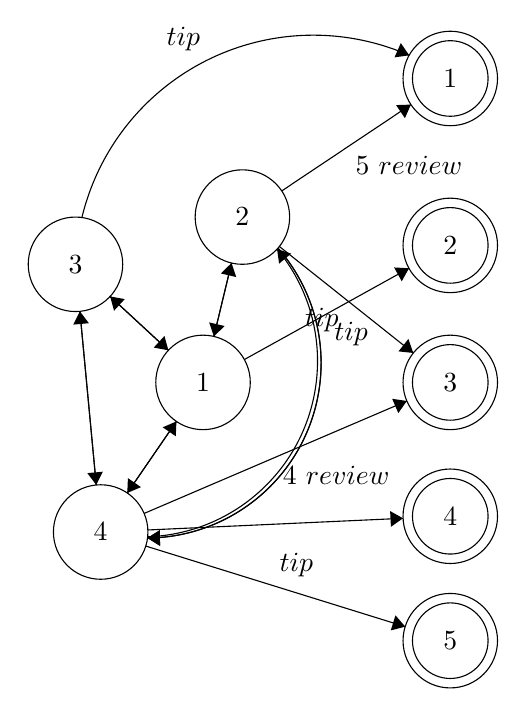
\begin{tikzpicture}[scale=0.2]
\tikzstyle{every node}+=[inner sep=0pt]
\draw [black] (28.4,-27.4) circle (3);
\draw (28.4,-27.4) node {$1$};
\draw [black] (30.9,-16.9) circle (3);
\draw (30.9,-16.9) node {$2$};
\draw [black] (20.3,-19.9) circle (3);
\draw (20.3,-19.9) node {$3$};
\draw [black] (21.9,-36.9) circle (3);
\draw (21.9,-36.9) node {$4$};
\draw [black] (44.1,-8.1) circle (3);
\draw (44.1,-8.1) node {$1$};
\draw [black] (44.1,-8.1) circle (2.4);
\draw [black] (44.1,-18.7) circle (3);
\draw (44.1,-18.7) node {$2$};
\draw [black] (44.1,-18.7) circle (2.4);
\draw [black] (44.1,-27.4) circle (3);
\draw (44.1,-27.4) node {$3$};
\draw [black] (44.1,-27.4) circle (2.4);
\draw [black] (44.1,-35.9) circle (3);
\draw (44.1,-35.9) node {$4$};
\draw [black] (44.1,-35.9) circle (2.4);
\draw [black] (44.1,-43.8) circle (3);
\draw (44.1,-43.8) node {$5$};
\draw [black] (44.1,-43.8) circle (2.4);
\draw [black] (33.4,-15.24) -- (41.6,-9.76);
\fill [black] (41.6,-9.76) -- (40.66,-9.79) -- (41.22,-10.62);
\draw (41.47,-13) node [below] {$5\mbox{ }review$};
\draw [black] (33.25,-18.77) -- (41.75,-25.53);
\fill [black] (41.75,-25.53) -- (41.44,-24.64) -- (40.81,-25.43);
\draw (35.94,-22.64) node [below] {$tip$};
\draw [black] (30.21,-19.82) -- (29.09,-24.48);
\fill [black] (29.09,-24.48) -- (29.77,-23.82) -- (28.79,-23.59);
\draw [black] (29.09,-24.48) -- (30.21,-19.82);
\fill [black] (30.21,-19.82) -- (29.53,-20.48) -- (30.51,-20.71);
\draw [black] (22.5,-21.94) -- (26.2,-25.36);
\fill [black] (26.2,-25.36) -- (25.95,-24.45) -- (25.27,-25.19);
\draw [black] (26.2,-25.36) -- (22.5,-21.94);
\fill [black] (22.5,-21.94) -- (22.75,-22.85) -- (23.43,-22.11);
\draw [black] (26.71,-29.88) -- (23.59,-34.42);
\fill [black] (23.59,-34.42) -- (24.46,-34.05) -- (23.63,-33.48);
\draw [black] (23.59,-34.42) -- (26.71,-29.88);
\fill [black] (26.71,-29.88) -- (25.84,-30.25) -- (26.67,-30.82);
\draw [black] (21.62,-33.91) -- (20.58,-22.89);
\fill [black] (20.58,-22.89) -- (20.16,-23.73) -- (21.15,-23.64);
\draw [black] (20.58,-22.89) -- (21.62,-33.91);
\fill [black] (21.62,-33.91) -- (22.04,-33.07) -- (21.05,-33.16);
\draw [black] (33.154,-18.866) arc (41.17132:-89.62681:11.106);
\fill [black] (24.87,-37.28) -- (25.67,-37.78) -- (25.66,-36.78);
\draw [black] (33.153,-18.867) arc (41.13512:-89.59061:11.108);
\fill [black] (24.87,-37.28) -- (25.67,-37.78) -- (25.66,-36.78);
\draw [black] (33.101,-18.926) arc (39.66688:-88.12237:11.16);
\fill [black] (33.1,-18.93) -- (33.23,-19.86) -- (34,-19.22);
\draw [black] (31.02,-25.95) -- (41.48,-20.15);
\fill [black] (41.48,-20.15) -- (40.53,-20.1) -- (41.02,-20.98);
\draw (37.8,-23.55) node [below] {$tip$};
\draw [black] (20.708,-16.933) arc (166.48658:66.25769:15.116);
\fill [black] (41.49,-6.63) -- (40.96,-5.85) -- (40.56,-6.76);
\draw (27.15,-6.41) node [above] {$tip$};
\draw [black] (24.9,-36.77) -- (41.1,-36.03);
\fill [black] (41.1,-36.03) -- (40.28,-35.57) -- (40.33,-36.57);
\draw [black] (24.76,-37.79) -- (41.24,-42.91);
\fill [black] (41.24,-42.91) -- (40.62,-42.19) -- (40.32,-43.15);
\draw (34.33,-39.78) node [above] {$tip$};
\draw [black] (24.66,-35.72) -- (41.34,-28.58);
\fill [black] (41.34,-28.58) -- (40.41,-28.44) -- (40.8,-29.35);
\draw (36.85,-32.7) node [below] {$4\mbox{ }review$};
\end{tikzpicture}
\caption{Proposed Complex Graph Models Based on Users, Reviews, Businesses, User-User Interactions, and Tips}
\label{fig:graph_complex_structure}
\end{figure}

\subsection{Predictive Models}
The rich meta-data about the network makes it quite interested to analyze, and opens up a lot of venues for possible improvements in terms of link prediction. We have multiple networks available for explorations, including \textit{user-user} network (based on friendships, comments, etc.), \textit{user-business} network, based on reviews given by a specific business to a user.

Furthermore, we also have the raw text of the Yelp Review as well as geographical information about the business and photos for some businesses, which opens the possibility of using moderns visual image recognition and natural language processing techniques to further extract node-level meta-data to incorporate into our model.

Concretely, we focus our work on predicting the rating that a user will assign a particular business. This problem has immediate and obvious utility: it would be useful to help users discover new businesses to visit (if the predicted rating is high) and also help business determine positive and negative trends. The dataset can be broken into three sets so we can train, evaluate, and test our models. One set will have edges, reviews, and information for businesses for a certain time $[t_0, t_1)$, the second set will have the edges created from $[t_1, t_2)$ and will be used to cross-validate our models and tune hyper-parameters, and the third set will he a hold out containing edges from $[t_2, t_3)$ and will be used for testing only.

\subsection{Network Structure}
Based on on previous work, we try a supervised learning model approach which will make use of both network-level features as well as node metadata. Let $G = (V,E)$ be our entire network spanning from $[t_0, t_3]$. We create $G_i = (V_i, E_i)$ for $0 \leq i \leq 2$ for each of the intervals mentioned above $[t_i, t_{i+1})$.

We extract the following set of topological network features, based on the literature:
\begin{itemize}
\item Afar-Adamic distance \cite{Adamic01friendsand}.
\item Following \cite{5562752}, we augment information using the bipartite structure of the graph.
\item We collapse the graph to generate positive and negative edges based on user-user interactions and extract user-level features that were helpful in predicting positive/negative edges in previous examples.
\item We extract other topological features mentioned above.
\end{itemize}

We also make use of the rich meta-data provided for each node as follows:
\begin{itemize}
\item Simple user features such as the number of hot compliments.
\item Other metrics for the user found in the Yelp Dataset.
\item Business metrics such as its category, whether it is open or not, and its postal code.
\item We concatenate reviews by the same user and use these as an input feature to an RNN for language extraction.
\item Similarly, we can concatenate reviews of business and use these for features relating to the business nodes.
\item We use photos (when available) as input features for the businesses by using transfer learning to transfer some.
\item There is additional data associate with each node which we can use and extract.
\end{itemize}

\section{Results and Discussion}
In this section, we present the results of our models.

\subsection{Summary Statistics}
We present some analysis on our networks defined above. 

\subsubsection{Users}
We present some overview of the user metadata. In Figure \ref{fig:user_characteristics}, we can see that multiple characteristics of the users follow a power-law degree distributions -- and not just the node degrees. This is to say that the distribution can be modelled as $P(k) \propto k^{-\gamma}$The power-law distribution is immediate evident in:

\begin{itemize}
\item Number of review -- we have a few users that write many rewiews and many users that write few reviews
\item Number of friends -- this means the network follows a true-power law distribution.
\item useful/funny/cool/fans -- this appears to demonstrate that social ranking/status also follows a power-law distribution in the Yelp social network. This trend is further demonstrated by Figure \ref{fig:user_compliment_distribution}.
\end{itemize} 

\begin{figure}[h!]
\centering
\includegraphics[width=0.5\textwidth]{../shared/figures/distribution_user_characteristics}
\caption{Frequency of countable user charatersitics -- the majority exhibit a powerlaw distributions}
\label{fig:user_characteristics}
\end{figure}

Furthermore, we can look at the averate rating given by users, across the network. The results are shown in a log plot in Figure \ref{fig:user_rating_distribution}.

\begin{figure}[h!]
\centering
\includegraphics[width=0.5\textwidth]{../shared/figures/average_user_rating_distribution}
\caption{Distribution of Average user Rating}
\label{fig:user_rating_distribution}
\end{figure}

We notice that the ratings tend to be inflated (3-5) stars being quite frequent, while 1-2 stars being very infrequent. Presumable this might be due to the fact that people do not frequent poor restaurants. The other aspect that is immediately apparent is the spikes at even numbered ratings -- this is likely due to users who have rated only one once, of which we have many.

\begin{figure}[h!]
\centering
\includegraphics[width=0.5\textwidth]{../shared/figures/compliement_type_distribution}
\caption{Distribution of Received user Compliments}
\label{fig:user_compliment_distribution}
\end{figure}

\subsubsection{Businesses}
We present some overview of the user metadata. In Figure \ref{fig:business_review_distribution}, we can see that the power-law distribution is also respected in the business side. Furthermore, we can also see that businesses tend to be rated quite highly, on average, with most businesses iether having in the range from 3-5 (see Figure \ref{fig:business_star_distribution}).

\begin{figure}[h!]
\centering
\includegraphics[width=0.5\textwidth]{../shared/figures/business_review_count_distribution}
\caption{Business Review Distribution}
\label{fig:business_review_distribution}
\end{figure}

\begin{figure}[h!]
\centering
\includegraphics[width=0.5\textwidth]{../shared/figures/business_star_distribution}
\caption{Business Average Star Distribution}
\label{fig:business_star_distribution}
\end{figure}

\subsection{Review Prediction}
In this section, we will compare the different methods utilized for review prediction. The methods include but are not limited to those discussed in the methods section above. We have yet to attempt making predictions, as this is a work-in-progress section.

We will likely evaluate the results using $RMSE$ between the predicted score and the actual score. So over our testing set $T$, we will calculate:
$$
RMSE = \sqrt{\frac{1}{|T|} \sum_{t \in T}(t - \hat{t})^2}
$$

\section{Future Work}

In the final report, we will present the results from training our end-to-end prediction model making use of both metadata and network structure features. We have yet to train a model on the entire data set. We will be using pre-trained deep-networks, such as VGGNet16 (for parsing images) and word2vec for parsing the natural language in the reviews.

\bibliography{../shared/references}{}
\bibliographystyle{plain}

\end{document}
